\documentclass[12pt,a4paper]{article}
\usepackage[utf8]{inputenc}
\usepackage{geometry}
\usepackage{graphicx}
\usepackage{amsmath}
\usepackage{hyperref}
\usepackage{lipsum}
\usepackage{longtable}
\usepackage{booktabs}
\usepackage{indentfirst}


% Page layout
\geometry{top=1in, bottom=1in, left=1in, right=1in}

% Title settings
\begin{document}
\begin{titlepage}
    \centering
    \vspace*{1cm}

    % Menambahkan logo atau gambar yang diinginkan di tengah
   

    {\LARGE \textbf{Deep Learning Course}}\\[0.5cm]
    {\Large \textbf{Final Project Report}}\\[1.5cm]

     
\includegraphics[width=0.5\textwidth]{images/Logo-Resmi-Unhas-2.png}\\[1cm] % Ganti dengan nama file gambar Anda
    
    % Daftar penulis
    \textbf{Disusun oleh:}\\[0.5cm]
    \begin{tabbing}
        \hspace{3cm} \= Aan Syawaluddin Adi Putra \hspace{3cm} \= H071221031 \kill
        \> Aan Syawaluddin Adi Putra \hspace{1cm} \= H071221031 \\
        \> Zabryna Andiny \hspace{3.15cm} \= H071221066 \\
        \> Khalizatul Jannah \hspace{2.8cm} \= H071221101 \\
    \end{tabbing}
    
    \vfill
    
    % Informasi universitas dan tanggal
    \textbf{Universitas Hasanuddin}\\
    \textbf{Makassar, Indonesia}\\[0.5cm]
    \textbf{\today}
    
\end{titlepage}


\tableofcontents
\newpage


\section{Introduction}

\subsection{Background \& Context}

Senam otak, atau yang dikenal sebagai \textit{brain gym}, merupakan serangkaian gerakan sederhana yang dirancang untuk meningkatkan fungsi kognitif, koordinasi motorik, dan kesehatan mental. Dengan melibatkan gerakan-gerakan yang mengaktifkan kedua belahan otak secara seimbang, \textit{brain gym} bertujuan untuk meningkatkan konsentrasi, daya ingat, dan kemampuan berpikir kritis. Aktivitas ini telah banyak digunakan dalam terapi pendidikan, rehabilitasi, dan pengembangan keterampilan kognitif pada berbagai kelompok usia.

Di era digital yang serba cepat, kemampuan otak untuk tetap fokus dan efektif dalam memproses informasi menjadi semakin penting. Dalam konteks ini, teknologi berbasis \textit{deep learning} menawarkan peluang besar untuk menganalisis gerakan \textit{brain gym} secara lebih mendalam. Namun, penelitian berbasis teknologi tentang \textit{brain gym} masih terbatas, terutama karena kurangnya \textit{dataset} standar yang dapat digunakan untuk melatih model pengenalan gerakan tubuh secara akurat.

\textit{Dataset} berkualitas tinggi diperlukan untuk mendukung penelitian dan pengembangan aplikasi yang dapat mengenali, menganalisis, dan merekomendasikan latihan \textit{brain gym} yang optimal berdasarkan kebutuhan individu. Dengan memanfaatkan \textit{dataset} ini, teknologi seperti \textit{pose estimation} dapat diterapkan untuk mempelajari efek gerakan terhadap fungsi kognitif, sekaligus membuka peluang untuk personalisasi latihan berdasarkan usia, kondisi fisik, atau kebutuhan spesifik lainnya.

\subsection{Problem Statement}
Meskipun \textit{brain gym} memiliki banyak manfaat yang diakui secara luas, terdapat sejumlah tantangan utama dalam penelitian dan pengembangan teknologi berbasis analisis gerakan ini, antara lain:

\begin{enumerate}
    \item \textbf{Ketiadaan Dataset Terstandar:} Belum ada \textit{dataset} terstandarisasi yang mencakup enam gerakan utama \textit{brain gym} yang dianggap paling efektif.
    \item \textbf{Keterbatasan Aksesibilitas Data:} \textit{Dataset} gerakan tubuh yang tersedia saat ini lebih berfokus pada aktivitas fisik kompleks, sehingga kurang relevan untuk analisis gerakan sederhana yang khas pada \textit{brain gym}.
    \item \textbf{Kurangnya Kompatibilitas dengan Teknologi Modern:} \textit{Dataset} yang ada sering kali tidak cocok untuk digunakan dalam model \textit{pose estimation} atau algoritma \textit{deep learning}, seperti \textit{OpenPose} atau \textit{MediaPipe}.
    \item \textbf{Sulitnya Personalisasi Latihan:} Tanpa \textit{dataset} yang terstruktur dan relevan, sulit untuk membuat aplikasi yang dapat mempersonalisasi latihan berdasarkan kebutuhan spesifik pengguna.
\end{enumerate}

\subsection{Objectives of the Research}
Proyek ini bertujuan untuk:

\begin{enumerate}
    \item Mengembangkan \textit{dataset} yang mencakup enam gerakan utama \textit{brain gym}: \textit{thumb side}, \textit{peace}, \textit{pistol}, \textit{little finger}, \textit{default}, dan \textit{back slap}.
    \item Menyediakan \textit{dataset} yang kompatibel dengan algoritma \textit{pose estimation}, seperti \textit{OpenPose} atau \textit{MediaPipe}.
    \item Membantu peneliti menganalisis efektivitas gerakan \textit{brain gym} terhadap peningkatan fungsi kognitif, koordinasi motorik, dan relaksasi.
    \item Menyediakan dasar untuk aplikasi yang dapat merekomendasikan latihan \textit{brain gym} berdasarkan profil pengguna.
\end{enumerate}

\newpage
\section{Related Works}

\subsection{Literature Review of Relevant Papers and Articles}
Brain Gym, atau Senam Otak, adalah serangkaian latihan yang terdiri dari 26 gerakan dasar yang bertujuan untuk meningkatkan fungsi kognitif seperti konsentrasi, memori, dan koordinasi motorik antara otak dan tubuh. Latihan ini membantu meningkatkan koordinasi mata dan tangan, meredakan ketegangan, serta meningkatkan fokus dan daya ingat. Program Brain Gym dibagi menjadi tiga dimensi utama: lateralitas (sinkronisasi otak kanan dan kiri), perhatian (peningkatan konsentrasi), dan pemusatan (pengendalian tindakan dan proses mental). Aktivitas ini tidak hanya memberi manfaat kognitif tetapi juga mendukung kesejahteraan psikologis.

Berbagai penelitian mengonfirmasi pentingnya latihan berbasis gerakan ini dalam meningkatkan fungsi otak dan kesejahteraan psikologis. Salah satunya adalah penelitian oleh Azizah et al. (2017) yang menunjukkan bahwa senam otak dapat meningkatkan fungsi kognitif dan mengurangi stres pada lansia. Senam otak membantu menyeimbangkan otak kanan dan kiri, yang berperan penting dalam pengendalian emosi dan logika, serta berkontribusi pada kesejahteraan psikologis lansia. Penelitian ini menyoroti bagaimana aktivitas fisik yang melibatkan gerakan dapat memperkuat koneksi saraf di otak, mendukung plastisitas otak, dan meningkatkan regulasi emosi.
Lebih lanjut, penelitian oleh Wei et al. (2024) dalam Personalized Daily Hand Movement Training Methods and Effects menunjukkan bahwa metode pelatihan gerakan tangan yang dipersonalisasi juga meningkatkan kesejahteraan subjektif individu dan kebahagiaan, sembari mengurangi emosi negatif. Metode ini menekankan pentingnya gamifikasi dalam rehabilitasi, yang relevansinya semakin jelas dalam konteks terapi berbasis gerakan, termasuk Brain Gym. Seperti yang ditemukan oleh Wei et al., pelatihan yang berfokus pada kebahagiaan dan keterlibatan peserta dapat meningkatkan hasil terapi secara signifikan.

Senada dengan ini, Siroya et al. (2021) menemukan bahwa latihan Brain Gym efektif dalam mengurangi stres, kecemasan, dan depresi pada mahasiswa, dengan fokus pada peningkatan konsentrasi dan memori. Penelitian ini menunjukkan bahwa latihan tersebut dapat memperbaiki persepsi psikologis, yang juga dipengaruhi oleh faktor eksternal seperti pengaturan waktu dan konsentrasi optimal. Hal ini mencerminkan pentingnya mempertimbangkan variabel eksternal dalam merancang program latihan seperti Brain Gym.

Dan untuk dari segi model kami melihat dari jurnal “Smart trainer: Combining video analysis and deep learning for efficient and accurate gym exercise classification and form correction” yang ditulis oleh Yogesh Kumar, Pratik Saria, Vikas Bhandari, Dinesh Kumar Vishwakarma pada tahun 2024, mengusulkan bawha pendekatan baru untuk mengenali dan mengklasifikasikan latihan kebugaran menggunakan deteksi pose manusia dengan Mediapipe dan LSTM, diikuti dengan pencocokan akurasi latihan menggunakan algoritma Hungaria dan kesamaan kosinus. Pendekatan yang diusulkan melibatkan penggunaan kombinasi teknologi mutakhir, termasuk visi komputer dan pembelajaran mendalam, untuk mengenali dan mengklasifikasikan berbagai latihan kebugaran secara akurat dan efisien. Studi ini menyajikan beberapa keuntungan dari pendekatan ini, termasuk kemampuan untuk memanfaatkan informasi temporal, ketahanan terhadap variasi pencahayaan, sudut kamera, dan oklusi, serta kemampuan untuk menangani berbagai macam latihan kebugaran. Hasil eksperimen menunjukkan bahwa pendekatan yang diusulkan mencapai akurasi tinggi dan mengungguli metode yang ada untuk pengenalan dan klasifikasi latihan kebugaran. Makalah ini juga membandingkan pendekatan yang diusulkan dengan teknik yang ada, menyoroti kekuatan dan efektivitas biayanya. Makalah ini diakhiri dengan menguraikan metodologi, termasuk pengumpulan dan pra-pemrosesan kumpulan data, ekstraksi landmark, pelatihan model LSTM, klasifikasi latihan, dan analisis kesamaan. Akhirnya, makalah ini membahas area penelitian masa depan yang potensial di bidang ini.


Namun, meskipun manfaat Brain Gym telah dibahas secara luas, tantangan utama dalam mengembangkan teknologi berbasis gerakan adalah menciptakan dataset yang mencakup variasi kondisi lingkungan, seperti pencahayaan, jarak, dan latar belakang yang berbeda. Dengan mengatasi tantangan ini, teknologi senam otak dapat dioptimalkan untuk meningkatkan akurasi pengenalan gerakan dalam berbagai situasi kehidupan nyata. Hal ini juga membuka peluang untuk integrasi teknologi AI dalam terapi berbasis gerakan, yang dapat meningkatkan efektivitas dalam mendukung kesehatan psikologis dan kognitif.


\subsection{Comparison of Different Approaches and Their Results}
Pada penelitian-penelitian yang disebutkan, terdapat berbagai pendekatan yang digunakan, masing-masing dengan tujuan dan metode yang sesuai dengan konteks penelitian mereka. Berikut adalah penjelasan tentang pendekatan-pendekatan yang digunakan dalam penelitian tersebut:

\begin{enumerate}
    \item Personalized Daily Living Hand Movement Training:
    \begin{itemize}
        \item Pendekatan : Menggunakan metode berbasis Happiness Memory Therapy (HMT) dan Positive Creation Mirror Theory (PCMT), yang dikombinasikan dengan pendekatan gamifikasi.

        \item Tujuan: Pendekatan ini bertujuan untuk melibatkan peserta dalam latihan gerakan tangan sehari-hari yang dipersonalisasi untuk meningkatkan kebahagiaan dan kreativitas mereka. Gamifikasi memberikan elemen permainan yang bertujuan untuk meningkatkan motivasi dan keterlibatan peserta selama pelatihan. Hal ini bisa meningkatkan efektivitas dalam meningkatkan keterampilan motorik serta kebahagiaan individu.
    \end{itemize}

    \item Improvement of Cognitive Function and Decrease the Level of Stress in the Elderly with Brain Gym:
    \begin{itemize}
        \item Pendekatan: Pendekatan ini menggunakan desain pre-experimental dengan metode one-group pretest-posttest.
        \item Tujuan: Pendekatan ini digunakan untuk mengukur perubahan dalam fungsi kognitif dan tingkat stres pada lansia setelah mengikuti latihan Brain Gym. Dengan menggunakan pretest dan posttest pada satu grup, penelitian ini bertujuan untuk melihat apakah ada peningkatan kognitif dan penurunan stres setelah intervensi yang diberikan. Ini adalah pendekatan eksperimental dasar yang memberikan gambaran awal tentang dampak suatu intervensi.
    \end{itemize}

    \newpage

    \item Brain Gym Exercises: An Approach in Improving Psychological Perception in Graduate Students:

    \begin{itemize}
        \item Pendekatan: Penelitian ini menggunakan metode pre-post interventional study dengan purposive sampling.
        \item Tujuan: Dalam penelitian ini, pendekatan pre-post digunakan untuk menilai perubahan dalam persepsi psikologis mahasiswa pascasarjana setelah mengikuti latihan Brain Gym. Purposive sampling dipilih untuk mengidentifikasi peserta yang dianggap relevan dengan tujuan penelitian, seperti mahasiswa yang mungkin mengalami stres atau tantangan psikologis tertentu. Dengan menggunakan pendekatan ini, peneliti dapat mengevaluasi efek latihan terhadap perubahan persepsi psikologis.
    \end{itemize}

\end{enumerate}

Membuat dataset untuk senam otak sangat penting karena adanya gap dalam penelitian yang ada, seperti kurangnya data terstruktur yang menggabungkan gerakan fisik dengan perubahan kognitif dan psikologis secara objektif. Penelitian sebelumnya hanya mengandalkan metode pretest-posttest atau observasional tanpa memanfaatkan teknologi canggih untuk mengukur gerakan tubuh secara real-time. Dengan menyediakan dataset yang mencakup gerakan tangan, kondisi kognitif, dan parameter psikologis peserta, kita dapat mengembangkan model yang lebih holistik dan terpersonalisasi untuk menilai efektivitas senam otak dalam meningkatkan fungsi kognitif dan mengurangi stres di berbagai kelompok usia dan latar belakang budaya.

\subsection{Justification for Chosen Methodology}
Proyek ini bertujuan untuk mengatasi keterbatasan dalam penelitian Brain Gym sebelumnya dengan mengembangkan dataset yang mencakup berbagai gerakan utama, seperti default, back slap, little finger, peace, pistol, dan thumb side. Dataset ini dirancang untuk mencakup gerakan tangan yang sederhana namun efektif dalam meningkatkan koordinasi, konsentrasi, dan keterlibatan mental.

Metodologi yang dipilih melibatkan perekaman gerakan melalui video, diikuti dengan anotasi gerakan untuk memastikan data yang dihasilkan kompatibel dengan berbagai aplikasi analisis data dan pembelajaran mesin. Dengan pendekatan ini, dataset yang dihasilkan tidak hanya mendukung penelitian lebih lanjut tetapi juga membuka peluang untuk pengembangan aplikasi berbasis teknologi yang dapat mempersonalisasi latihan berdasarkan kebutuhan pengguna.

Pendekatan ini memiliki beberapa keunggulan utama. Pertama, data yang dihasilkan lebih terstruktur dan terstandarisasi, memungkinkan analisis dalam skala besar. Kedua, penggunaan teknologi memungkinkan pengukuran yang lebih objektif dan efisien dibandingkan dengan metode manual. Ketiga, dataset ini dapat digunakan untuk mendukung berbagai aplikasi di bidang pendidikan, terapi fisik, dan kesehatan mental, memberikan manfaat yang lebih luas bagi masyarakat.

Dengan metodologi ini, proyek diharapkan dapat melengkapi kekurangan dalam literatur sebelumnya dan memberikan kontribusi yang signifikan terhadap pemahaman tentang dampak Brain Gym. Selain itu, pengembangan dataset berbasis teknologi ini dapat menjadi langkah awal menuju pendekatan yang lebih modern dan berbasis data dalam menganalisis hubungan antara gerakan, kognisi, dan kesejahteraan psikologis.


\newpage

\section{Dataset and Materials}
\subsection{Source of the dataset}
Dalam pengembangan dataset Brain Gym, data untuk proyek ini diperoleh dengan merekam gerakan tangan langsung menggunakan perangkat kamera seperti webcam atau kamera smartphone. Fokus utama perekaman adalah enam gerakan tangan spesifik: default, back slap, little finger, peace, pistol, dan thumb side. Setiap gerakan direkam dalam durasi 2 detik, dengan variasi pada sudut tangan, kecepatan gerakan, dan jarak tangan terhadap kamera untuk memastikan keragaman data. Proses perekaman dilakukan di lingkungan yang terkendali, dengan pencahayaan yang cukup dan latar belakang yang sederhana untuk meminimalkan gangguan visual, memastikan data yang diperoleh berkualitas tinggi. 

Setelah pengambilan data, video yang dihasilkan diunggah ke platform RoboFlow untuk anotasi dan pelabelan, dengan setiap gerakan diberi kategori yang sesuai. Penggunaan RoboFlow memungkinkan pengelompokan data ke dalam kategori pelatihan, validasi, dan pengujian, yang penting untuk membangun model yang lebih akurat. Pengumpulan data secara langsung ini memberikan kontrol penuh terhadap kualitas dan relevansi dataset, memungkinkan adaptasi sesuai kebutuhan model dan mengoptimalkan analisis gerakan tangan dalam proyek ini.

\begin{table}[ht]
    \centering
    \begin{tabular}{|c|c|c|}
        \hline
        \textbf{Kelas Dataset} & \textbf{Jumlah Dataset (Video)} & \textbf{Durasi} \\ \hline
        default & 50 video & 2 detik/video \\ \hline
        peace & 20 video & 2 detik/video \\ \hline
        pistol & 26 video & 2 detik/video \\ \hline
        thumb\_side & 40 video & 2 detik/video \\ \hline
        little\_finger & 20 video & 2 detik/video \\ \hline
        back\_slap & 31 video & 2 detik/video \\ \hline
    \end{tabular}
    \caption{Detail Jumlah Dataset}
    \label{tab:dataset}
\end{table}

\subsection{Preprocessing Steps}
Langkah-langkah preprocessing dataset \textit{Brain Gym}, diantaranya:

\begin{itemize}
    \item \textbf{Ekstraksi Frame:} 
    Video yang direkam diunggah ke \textit{RoboFlow} dan diproses menjadi serangkaian frame. Setiap video dipisah menjadi gambar-gambar statis yang mewakili momen tertentu dalam gerakan tangan. Langkah ini memungkinkan model untuk menganalisis gambar individu, yang lebih mudah diproses dalam algoritma pembelajaran mesin.
    
    \item \textbf{Anotasi dengan RoboFlow:} 
    Setiap frame diberi label sesuai jenis gerakan tangan yang ditampilkan, seperti \textit{default}, \textit{back slap}, \textit{little finger}, \textit{peace}, \textit{pistol}, dan \textit{thumb side}. \textit{RoboFlow} mempermudah proses ini dengan alat anotasi otomatis yang memungkinkan pelabelan data secara lebih efisien.
    
    \item \textbf{Ekspor Dataset:} 
    Pada tahap ekspor dataset, setelah proses anotasi selesai, dataset yang telah dianotasi di \textit{RoboFlow} diekspor dalam format COCO (\textit{Common Objects in Context}). Format ini menghasilkan file JSON yang berisi informasi lengkap mengenai gambar dan anotasi gerakan tangan. Setiap gambar memiliki metadata terkait, seperti kategori gerakan (misalnya, \textit{"peace"}, \textit{"thumb side"}), dan posisi koordinat untuk setiap gerakan tangan yang diidentifikasi dalam bentuk \textit{bounding box}. File JSON ini memungkinkan integrasi langsung dengan model \textit{deep learning} dan analisis lebih lanjut menggunakan framework seperti \textit{TensorFlow} atau \textit{PyTorch}.
\end{itemize}

\begin{center}
    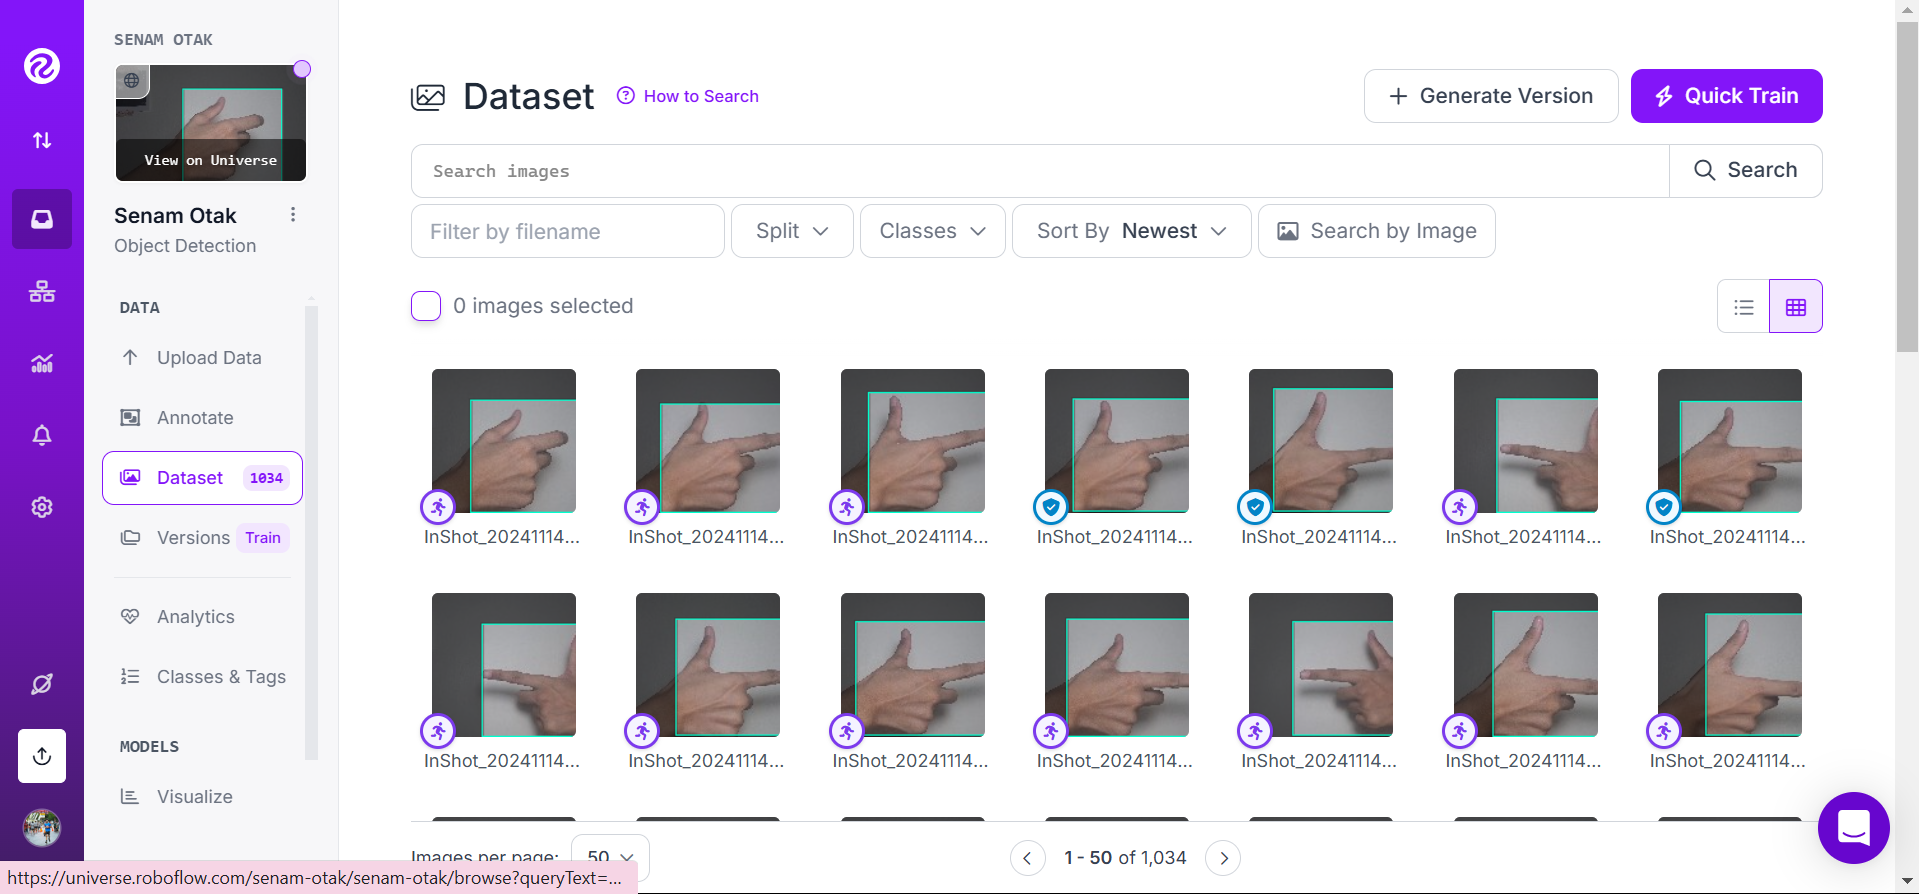
\includegraphics[width=0.9\textwidth]{images/1.png}
\end{center}

\begin{center}
    Gambar 1.  Anotasi dengan RoboFlow
\end{center}

\begin{table}[ht]
\centering
\begin{tabular}{|l|l|l|}
\hline
\textbf{Kelas Dataset} & \textbf{Jumlah Dataset (Video)} & \textbf{Jumlah Anotasi (Gambar)} \\ \hline
default       & 50 video  & 313 gambar  \\ \hline
peace         & 20 video  & 302 gambar  \\ \hline
pistol        & 26 video  & 314 gambar  \\ \hline
thumb\_side   & 40 video  & 300 gambar  \\ \hline
little\_finger & 20 video  & 298 gambar  \\ \hline
back\_slap    & 31 video  & 301 gambar  \\ \hline
\textbf{Total} & \textbf{187 video} & \textbf{1.828 gambar} \\ \hline
\end{tabular}
\caption{Detail Jumlah Dataset dan Anotasi}
\label{tab:dataset}
\end{table}

\subsection{Features and labels}
Dalam dataset ini, fitur terdiri dari gambar frame yang diambil dari video gerakan tangan yang telah direkam. Setiap gambar memiliki dimensi tertentu, misalnya 224x224 piksel, agar sesuai dengan kebutuhan model deep learning seperti CNN (Convolutional Neural Network). Fitur-fitur ini mewakili visual dari setiap gerakan tangan yang diobservasi.

Sedangkan label mencakup kategori gerakan tangan yang terdiri dari enam jenis gerakan, yaitu: default, back slap, little finger, peace, pistol, dan thumb side. Setiap gambar diberi label sesuai dengan gerakan yang terekam pada frame tersebut, yang digunakan untuk melatih model agar dapat mengidentifikasi gerakan dengan akurat.

\begin{center}
    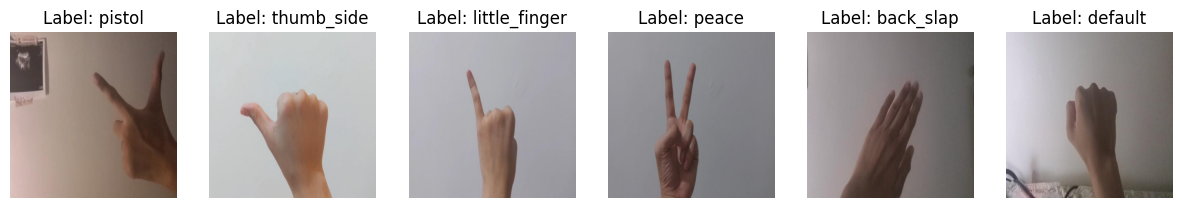
\includegraphics[width=0.9\textwidth]{images/2.png}
\end{center}

\begin{center}
    Gambar 2. Labeling Data
\end{center}

Tools, Libraries, and Frameworks digunakan untuk mendukung seluruh proses pengolahan data dan pengembangan model:
\begin{enumerate}
    \item Camera Tools: Digunakan untuk merekam video gerakan tangan. Perangkat kamera yang digunakan bisa berupa kamera smartphone atau webcam untuk memastikan perekaman yang efisien dan berkualitas.
    \item Google Collab: 
    \begin{center}
        
\includegraphics[width=0.2\textwidth]{images/3.png}
    \end{center}

    \begin{center}
        Gambar 3. Google Collab
    \end{center}
    Menggunakan Google Collab sebagai platform berbasis cloud untuk menulis, menjalankan, dan mempercepat kode, memanfaatkan dukungan GPU atau TPU gratis untuk meningkatkan efisiensi kerja.

    \item RoboFlow :
    \begin{center}
        
\includegraphics[width=0.2\textwidth]{images/4.png}
    \end{center}

    \begin{center}
        Gambar 4. Roboflow
    \end{center}
    Platform berbasis cloud yang digunakan untuk anotasi dataset dan preprocessing. RoboFlow menyediakan alat untuk label otomatis dan mempermudah pengelolaan dataset dalam berbagai format, seperti COCO dan TFRecord.

    \newpage
    \item TensorFlow/Keras: 
    \begin{center}
        
\includegraphics[width= 0.3\textwidth]{images/5.png}
    \end{center}
    \begin{center}
        Gambar 5. TensorFlow
    \end{center}
    Framework yang digunakan untuk membangun dan melatih model deep learning, terutama CNN (Convolutional Neural Networks) untuk ekstraksi fitur visual dari video dan LSTM untuk analisis temporal dari gerakan.

    \item Matplotlib dan Seaborn: 
    \begin{center}
        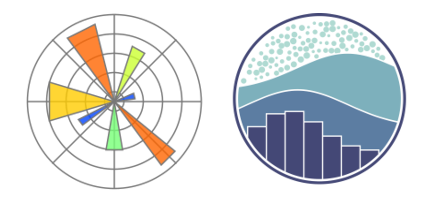
\includegraphics[width=0.45\textwidth]{images/6.png}
    \end{center}
    \begin{center}
        Gambar 6. Matplotlib dan Seaborn
    \end{center}

    Digunakan untuk visualisasi data dan hasil model. Matplotlib membantu dalam membuat grafik untuk analisis data dan kinerja model, sementara Seaborn digunakan untuk visualisasi statistik lebih lanjut, seperti distribusi data atau korelasi antar fitur
\end{enumerate}

\newpage

\section{Result and Discussion}
\subsection{Performance metrics}
Metrik kinerja mencakup : 
\begin{table}[ht]
\centering
\begin{tabular}{|l|c|c|c|c|}
\hline
\textbf{Label} & \textbf{Precision} & \textbf{Recall} & \textbf{F1-score} & \textbf{Support} \\ \hline
back\_slap     & 1.00              & 1.00            & 1.00              & 59              \\ \hline
default        & 1.00              & 1.00            & 1.00              & 63              \\ \hline
little\_finger & 1.00              & 1.00            & 1.00              & 62              \\ \hline
peace          & 1.00              & 1.00            & 1.00              & 62              \\ \hline
pistol         & 1.00              & 1.00            & 1.00              & 62              \\ \hline
thumb\_side    & 1.00              & 1.00            & 1.00              & 61              \\ \hline
\textbf{Accuracy}    &                    &                 & {1.00}     & {369}     \\ \hline
\textbf{Macro Avg}    & 1.00              & 1.00            & 1.00              & 369             \\ \hline
\textbf{Weighted Avg} & 1.00              & 1.00            & 1.00              & 369             \\ \hline
\end{tabular}
\caption{Classification Report}
\label{tab:classification_report}
\end{table}

\begin{center}
    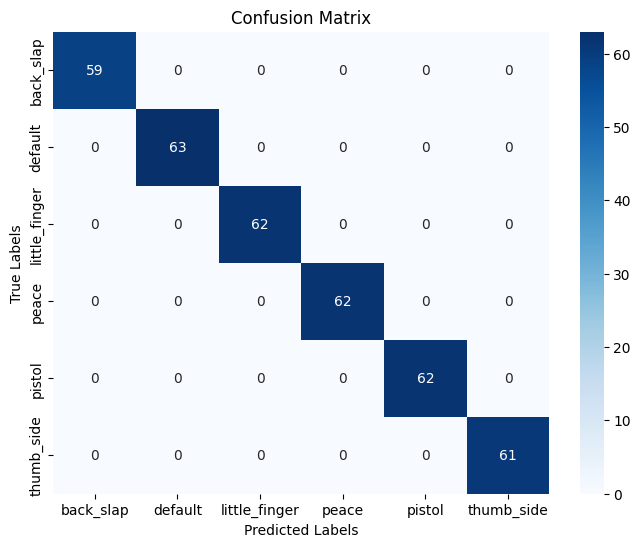
\includegraphics[width=0.9\textwidth]{images/7.png}
\end{center}
\begin{center}
    Gambar 7. Confusion Matrix
\end{center}

Hasil evaluasi menunjukkan bahwa model klasifikasi memiliki kinerja yang sempurna pada dataset ini. Semua metrik evaluasi, yaitu precision, recall, dan F1-score, memiliki nilai \textbf{1.00} untuk setiap kelas, yang mengindikasikan bahwa model mampu memprediksi semua instance dengan benar tanpa adanya kesalahan. Precision yang sempurna menunjukkan tidak ada prediksi positif yang salah (false positives), sedangkan recall yang sempurna memastikan bahwa tidak ada instance dari kelas sebenarnya yang terlewatkan (false negatives). Hal ini sesuai dengan confusion matrix sebelumnya, di mana semua nilai berada pada diagonal utama, tanpa kesalahan klasifikasi. Selain itu, rata-rata metrik baik secara makro maupun berbobot juga bernilai \textbf{1.00}, yang memperkuat kesimpulan bahwa model berhasil menangani dataset dengan sangat baik. Namun, meskipun hasil ini sangat baik, performa ini perlu diuji lebih lanjut pada dataset baru untuk memastikan kemampuan model dalam generalisasi pada data di luar dataset pelatihan.

\begin{table}[ht]
\centering
\begin{tabular}{|c|c|}
\hline
\textbf{Metric} & \textbf{Value} \\ \hline
Test Loss       & 0.2445         \\ \hline
Test Accuracy   & 0.9962         \\ \hline
\end{tabular}
\caption{Test Metrics}
\label{tab:test_metrics}
\end{table}

Pada tahap validasi, model menunjukkan \textbf{validation loss} sebesar 0.2445 dan \textbf{validation accuracy} sebesar 99.62\%. Validation loss yang rendah menunjukkan bahwa kesalahan prediksi model pada data validasi sangat kecil, sementara validation accuracy yang hampir sempurna mengindikasikan bahwa model dapat mengklasifikasikan hampir semua data validasi dengan benar. Konsistensi hasil ini dengan metrik evaluasi lainnya menguatkan bahwa model memiliki performa yang sangat tinggi. Namun, meskipun hasil ini sangat baik, diperlukan pengujian lebih lanjut menggunakan dataset independen untuk memastikan bahwa model mampu melakukan generalisasi dengan baik pada data di luar dataset pelatihan.

\subsection{Visualization of result}
\begin{center}
    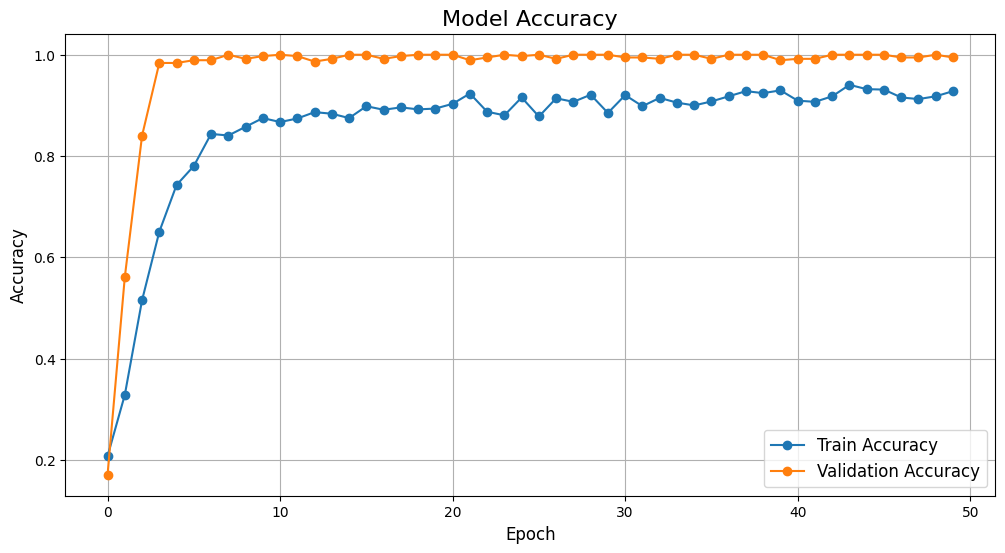
\includegraphics[width=1.0\textwidth]{images/8.png}
\end{center}

\begin{center}
    Gambar 8. Model Akurasi sebelum Dioptimasi
\end{center}

Grafik ini menunjukkan hubungan antara jumlah epoch dengan akurasi model sebelum optimasi dilakukan. Pada grafik, garis biru mewakili akurasi pada data pelatihan (train accuracy), sedangkan garis oranye mewakili akurasi pada data validasi (validation accuracy). Pada awal pelatihan, akurasi meningkat tajam untuk kedua data, namun setelah beberapa epoch, tren keduanya mulai stabil. Akurasi validasi cenderung lebih tinggi dibandingkan akurasi pelatihan di sebagian besar epoch, yang menunjukkan kemungkinan adanya regularisasi atau mekanisme lain yang membuat model lebih general terhadap data yang tidak dilatih. Namun, hal ini juga bisa mengindikasikan bahwa model belum sepenuhnya mempelajari pola dalam data pelatihan secara optimal. Secara keseluruhan, grafik ini mencerminkan performa model yang cukup baik, tetapi masih dapat ditingkatkan dengan optimasi lebih lanjut, seperti tuning hyperparameter atau arsitektur model.

\begin{center}
    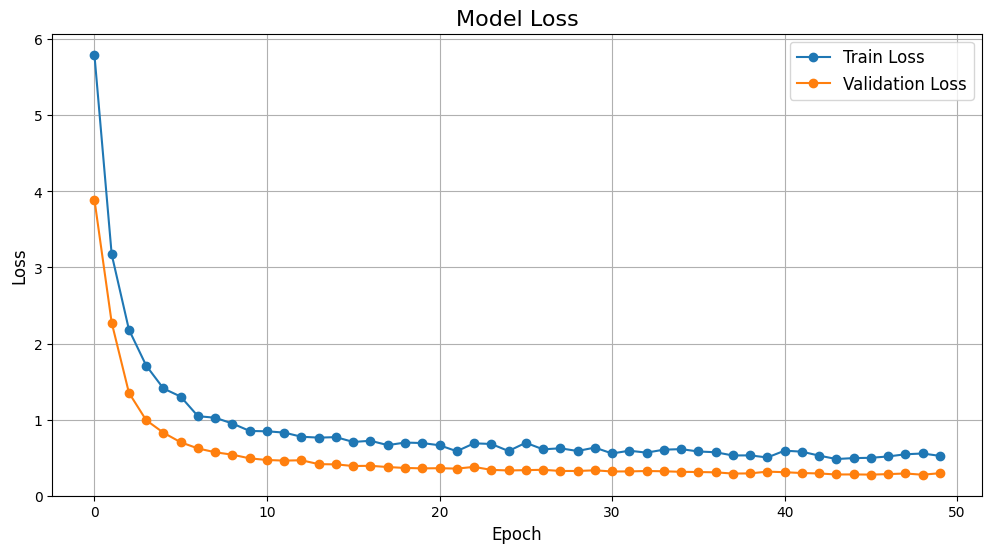
\includegraphics[width=1\textwidth]{images/9.png}
\end{center}

\begin{center}
    Gambar 9. Model Loss sebelum Optimasi
\end{center}

Grafik ini menunjukkan hubungan antara jumlah epoch dengan loss model (kerugian) selama proses pelatihan dan validasi. Garis biru mewakili train loss, yaitu kerugian yang dihitung pada data pelatihan, sementara garis oranye mewakili validation loss, yaitu kerugian pada data validasi.

Pada awal pelatihan, baik train loss maupun validation loss memiliki nilai yang cukup tinggi, yang menunjukkan bahwa model belum memahami pola dalam data. Seiring bertambahnya epoch, keduanya menurun secara signifikan, yang mencerminkan bahwa model semakin mampu mempelajari pola dalam data. Namun, setelah beberapa epoch, train loss menjadi relatif stabil tetapi lebih tinggi dibandingkan validation loss. Hal ini menunjukkan bahwa model mungkin terlalu sederhana atau ada regularisasi yang mencegah overfitting. Validation loss yang lebih rendah dibandingkan train loss juga dapat mengindikasikan bahwa model generalisasi dengan baik terhadap data yang tidak dilatih.

Grafik ini menunjukkan bahwa pelatihan berhasil mengurangi loss hingga mencapai titik stabil pada sekitar epoch ke-10. Meski begitu, perbedaan antara train loss dan validation loss dapat menjadi indikasi bahwa model masih dapat ditingkatkan melalui optimasi parameter atau pengujian arsitektur model yang lebih kompleks.

\begin{center}
    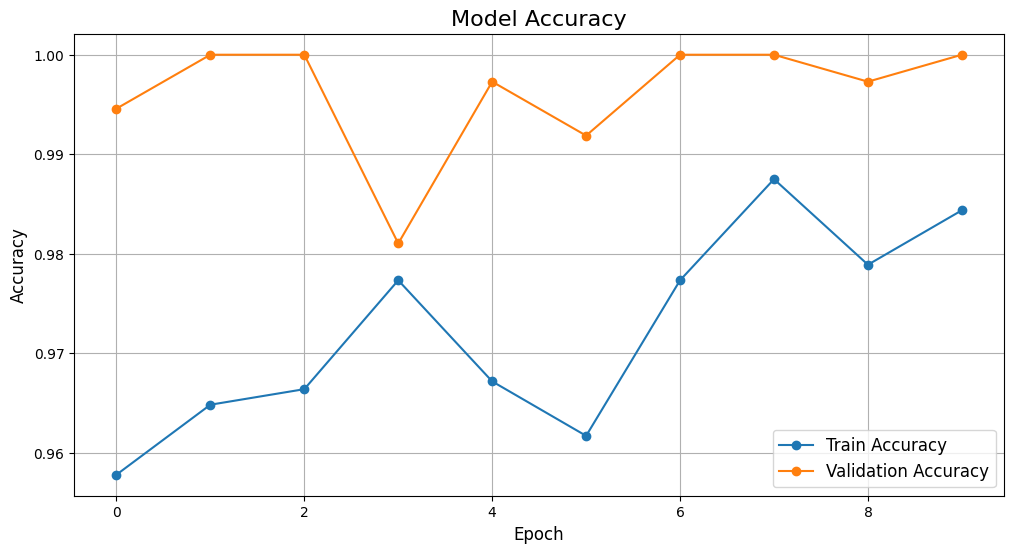
\includegraphics[width=1.0\textwidth]{images/10.png}
\end{center}

\begin{center}
    Gambar 10. Model Akurasi setelah Optimasi
\end{center}

Grafik ini menunjukkan akurasi model setelah dilakukan optimasi selama beberapa epoch. Garis biru mewakili \textbf{train accuracy} (akurasi pada data pelatihan), sementara garis oranye mewakili \textbf{validation accuracy} (akurasi pada data validasi).

Setelah optimasi, \textbf{validation accuracy} menunjukkan nilai yang sangat tinggi, mendek-ati 1 (100\%), dengan sedikit fluktuasi. Ini menunjukkan bahwa model memiliki performa yang sangat baik pada data validasi, mencerminkan kemampuan generalisasi yang optimal. Di sisi lain, \textbf{train accuracy} meningkat secara bertahap dan menunjukkan pola fluktuasi kecil tetapi cenderung menuju nilai yang lebih tinggi. Meski begitu, train accuracy masih sedikit lebih rendah dibandingkan validation accuracy.

Perbedaan kecil antara train accuracy dan validation accuracy menunjukkan bahwa model mampu belajar dengan baik dari data pelatihan tanpa mengalami overfitting. Optimasi yang dilakukan telah meningkatkan performa model, baik pada data pelatihan maupun data validasi. Grafik ini mengindikasikan bahwa model telah mencapai akurasi yang tinggi dengan generalisasi yang baik.

\begin{center}
    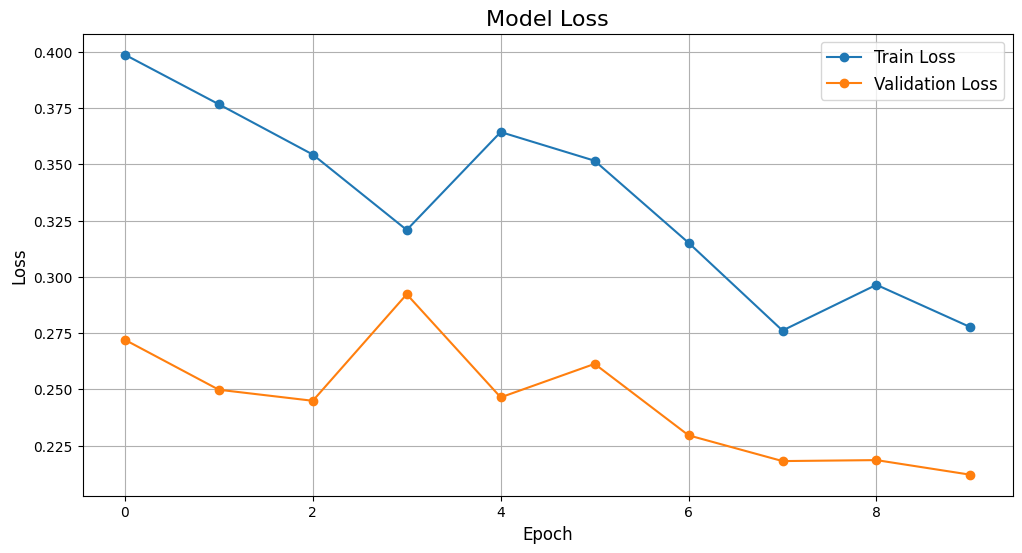
\includegraphics[width=1.0\textwidth]{images/11.png}
\end{center}

\begin{center}
    Gambar 11. Model Loss setelah Optimasi
\end{center}

Grafik ini menggambarkan perubahan nilai loss model selama proses pelatihan dan validasi berdasarkan jumlah epoch. Pada sumbu horizontal (X) ditampilkan jumlah epoch, yang menunjukkan berapa kali model melalui seluruh data pelatihan. Sedangkan sumbu vertikal (Y) menunjukkan nilai loss, yaitu ukuran seberapa besar kesalahan prediksi model. Nilai loss yang lebih kecil menunjukkan model yang lebih akurat.

Garis biru mewakili train loss, yaitu nilai loss yang dihitung dari data pelatihan. Nilai ini secara bertahap menurun seiring bertambahnya epoch, yang menandakan bahwa model semakin baik dalam belajar dari data pelatihan. Sementara itu, garis oranye menunjukkan validation loss, yang dihitung dari data validasi untuk mengevaluasi kinerja model pada data yang tidak terlihat selama pelatihan.

Pada grafik ini, validation loss juga cenderung menurun, meskipun mengalami sedikit fluktuasi di tengah proses pelatihan. Tren ini menunjukkan bahwa model tidak mengalami overfitting yang signifikan, di mana model hanya bekerja baik pada data pelatihan tetapi buruk pada data validasi. Dengan demikian, grafik ini mengindikasikan bahwa proses pelatihan berjalan dengan stabil dan model menunjukkan kinerja yang baik.

\subsection{Discussion of result}
Hasil evaluasi model klasifikasi pada dataset senam otak menunjukkan kinerja yang sangat baik, dengan semua metrik evaluasi, yang mencakup precision, recall, dan F1-score mencapai nilai 1.00 untuk setiap kelas. Hal ini menandakan bahwa model berhasil memprediksi semua instance dengan sangat akurat tanpa kesalahan. Precision yang sempurna menunjukkan bahwa tidak ada prediksi positif yang salah (false positives), sementara recall yang sempurna memastikan bahwa tidak ada instance dari kelas sebenarnya yang terlewatkan (false negatives). Hasil ini mencerminkan kemampuan model yang sangat baik dalam memahami pola gerakan dalam dataset ini.

Selain itu, nilai validation accuracy yang sangat tinggi (99.62\%) dan validation loss yang rendah (0.2445) menunjukkan bahwa model dapat menggeneralisasi dengan baik pada data yang belum pernah dilihat sebelumnya, yang sangat penting dalam aplikasi dunia nyata. Namun, meskipun hasil ini sangat baik, performa model perlu diuji lebih lanjut dengan dataset yang lebih besar atau dataset yang berbeda untuk memastikan kemampuan generalisasi yang lebih luas.

Ketika dibandingkan dengan penelitian lain yang relevan, seperti "Smart Trainer Using Deep Learning", terdapat beberapa perbedaan signifikan. Pada proyek tersebut, model berfokus pada klasifikasi gerakan olahraga berbasis video yang melibatkan berbagai variasi gerakan dan sudut kamera, yang bisa mempengaruhi akurasi model. Mereka melaporkan akurasi yang baik, tetapi performa menurun saat menangani gerakan yang kompleks atau data yang kurang berkualitas. Sementara itu, model dalam penelitian ini berfokus pada dataset senam otak yang lebih terstruktur, dengan gerakan-gerakan spesifik dan terbatas. Hasil evaluasi penelitian ini menunjukkan precision, recall, dan F1-score yang sempurna, yang mengindikasikan bahwa model dapat mengenali pola gerakan dengan sangat baik.

Meskipun model ini sangat efektif untuk dataset yang terstruktur dengan baik dan memiliki gerakan yang spesifik, ada beberapa aspek yang perlu diperhatikan untuk mening- katkan performa lebih lanjut. Ukuran Dataset menjadi salah satu faktor penting, karena dataset yang digunakan relatif kecil. Untuk meningkatkan kemampuan generalisasi dan menghindari overfitting, pengujian pada dataset yang lebih besar atau dengan variasi gerakan yang lebih banyak sangat disarankan. Selain itu, ketersediaan data baru perlu diperhatikan untuk memverifikasi apakah model ini dapat menggeneralisasi pada data yang tidak terlihat sebelumnya. Ini penting untuk memastikan bahwa model tidak hanya bekerja dengan baik pada dataset pelatihan, tetapi juga dapat diterapkan di dunia nyata. Terakhir, peningkatan arsitektur model dapat dilakukan dengan penerapan teknik augmentasi data atau penggunaan model yang lebih kompleks, seperti transfer learning, untuk meningkatkan kemampuan model dalam mengenali variasi gerakan yang lebih halus.

\newpage
\section{ Conclusion}
Penelitian ini berhasil mengembangkan dataset senam otak (Brain Gym) dengan pendekatan berbasis teknologi, mencakup enam gerakan tangan spesifik yang dianotasi secara sistematis menggunakan RoboFlow. Dataset ini dianalisis menggunakan model deep learning berbasis CNN dan LSTM untuk mengklasifikasikan gerakan tangan dengan tingkat akurasi tinggi.

Hasil evaluasi menunjukkan performa model yang sangat baik, dengan nilai precision, recall, dan F1-score mencapai 1.00 untuk setiap kelas. Validation accuracy sebesar 99.62\% dan validation loss sebesar 0.2445 mengindikasikan kemampuan model dalam mengenali pola secara akurat sekaligus melakukan generalisasi terhadap data yang tidak dilatih. Selain itu, grafik performa menunjukkan tren stabil dalam akurasi dan penurunan loss, menandakan proses pelatihan berjalan optimal.

Namun, penelitian ini juga mencatat beberapa potensi indikasi \textbf{overfitting}. Pada beberapa titik pelatihan, validation accuracy lebih tinggi dibandingkan train accuracy, yang dapat menunjukkan regularisasi yang mencegah overfitting tetapi juga menimbulkan pertanyaan apakah model sepenuhnya memahami data pelatihan. Meskipun perbedaan ini kecil, perlu diuji lebih lanjut dengan dataset baru untuk memastikan bahwa model tidak hanya cocok pada dataset yang ada tetapi juga dapat menggeneralisasi pada data yang lebih kompleks.

Oleh karena itu, penelitian di masa depan disarankan untuk:
\begin{enumerate}
    \item Menggunakan dataset yang lebih besar dan bervariasi untuk menguji kemampuan model dalam mengenali gerakan yang lebih kompleks.
    \item Mengimplementasikan teknik augmentasi data atau transfer learning untuk meningka-tkan akurasi dan kemampuan model dalam menangani variasi gerakan.
    \item Menguji model pada aplikasi dunia nyata untuk memvalidasi kinerjanya dalam skenario praktis.
\end{enumerate}

Penelitian ini memberikan kontribusi signifikan dalam menyediakan dataset terstruktur untuk analisis gerakan tangan serta menunjukkan potensi besar teknologi pembelajaran mesin untuk mendukung aplikasi dalam pendidikan, terapi fisik, dan kesehatan mental. Pengembangan lebih lanjut diperlukan untuk memastikan kemampuan generalisasi yang lebih baik dan penerapan di dunia nyata.

\newpage
\bibliographystyle{plain}
\begin{thebibliography}{9}

\bibitem{Kumar2024} Yogesh Kumar, Pratik Saria, Vikas Bhandari, Dinesh Kumar Vishwakarma, "Smart trainer: Combining video analysis and deep learning for efficient and accurate gym exercise classification and form correction," 2024.

\bibitem{MDPI2024} MDPI, "Personalized Daily Hand Movement Training Methods and Effects: A Case Study," \textit{MDPI}, https://www.mdpi.com/2076-3417/14/12/5297.

\bibitem{IJNMS2024} "View of The Improvement of Cognitive Function and Decrease the Level of Stress in the Elderly with Brain Gym," \textit{INTERNATIONAL JOURNAL OF NURSING AND MIDWIFERY SCIENCE (IJNMS)}, https://www.jknusantara.com/index.php/ijnms/article/view/33/4.

\bibitem{JMPAS2021} "Brain gym exercises: an approach in improving the psychological perception in graduate students," \textit{JMPAS}, September-October 2021, https://jmpas.com/admin/assets/article\_issue/1637781336JMPAS\_SEPTEMBER-OCTOBER\_2021.pdf.

\end{thebibliography}


\end{document}
